\documentclass[12pt,landscape]{exam}
\usepackage[hon]{template-for-exam}
\footer{}{}{}
\header{}{}{}

\usepackage{tikz}
\usetikzlibrary{shadings,decorations.pathmorphing,arrows.meta,patterns}
\tikzset{f/.append style={-{Stealth[length=3mm,width=2mm]}}}

\shadedsolutions
%\printanswers

\def\mystrut{\protect\rule[-2.2ex]{0ex}{2.2ex}} 
\qformat{ \textbf{Task \#\thequestion}
  \ifthenelse{\equal{\thequestion}{\thequestiontitle}}
    {}
    {: \emph{\thequestiontitle}}
  \mystrut  \hfill}

\newcommand{\hforce}[2]
{
  \draw[f] (a) -- ++(#1, 0) 
        node[anchor=south] {#2};
}
\newcommand{\vforce}[2]
{
  \draw[f] (a) -- ++(0, #1) 
        node[anchor=west] {#2};
}

\begin{document}
\begin{questions}

\Large

\question 
  In each of the free-body diagrams below, calculate the 
  {\bf magnitude} and {\bf direction} of the net force 
  and draw it.


  \begin{center}  
    \begin{tikzpicture}[scale=0.6]
      \newcommand{\createFBD}[1]
        {
          \filldraw (a) circle [radius=0.175];
          \path (a) node {} 
            + (-4,2.5) node {#1} ;
        }

      \begin{scope}
        \node (a) at (0,0) {};
        \createFBD{(a)}
        \vforce{ 2}{\SI{18}{\newton}}
        \vforce{-2}{\SI{18}{\newton}}

      \end{scope}

      \begin{scope}
        \node (a) at (9,0) {};
        \createFBD{(b)}
        \vforce{  2  }{\SI{40}{\newton}}
        \vforce{-1.25}{\SI{24}{\newton}}
      \end{scope}

      \begin{scope}
        \node (a) at (18,0) {};
        \createFBD{(c)}
        \vforce{ 2}{\SI{5}{\newton}}
        \vforce{-2}{\SI{5}{\newton}}
        \hforce{ 3}{\SI{7}{\newton}}
        \hforce{-3}{\SI{7}{\newton}}
      \end{scope}

      \begin{scope}
        \node (a) at (27,0) {};
        \createFBD{(d)}
        \vforce{  2 }{\SI{17}{\newton}}
        \vforce{ -2 }{\SI{17}{\newton}}
        \hforce{  3 }{\SI{32}{\newton}}
        \hforce{-1.5}{\SI{14}{\newton}}
      \end{scope}
    \end{tikzpicture}
  \end{center}

\vs \hrule \vs
      
\question 
  In each of the free-body diagrams below, the net force 
  is given, but one or more of the applied forces is 
  missing.  Find the missing forces.

  \begin{EnvUplevel}
    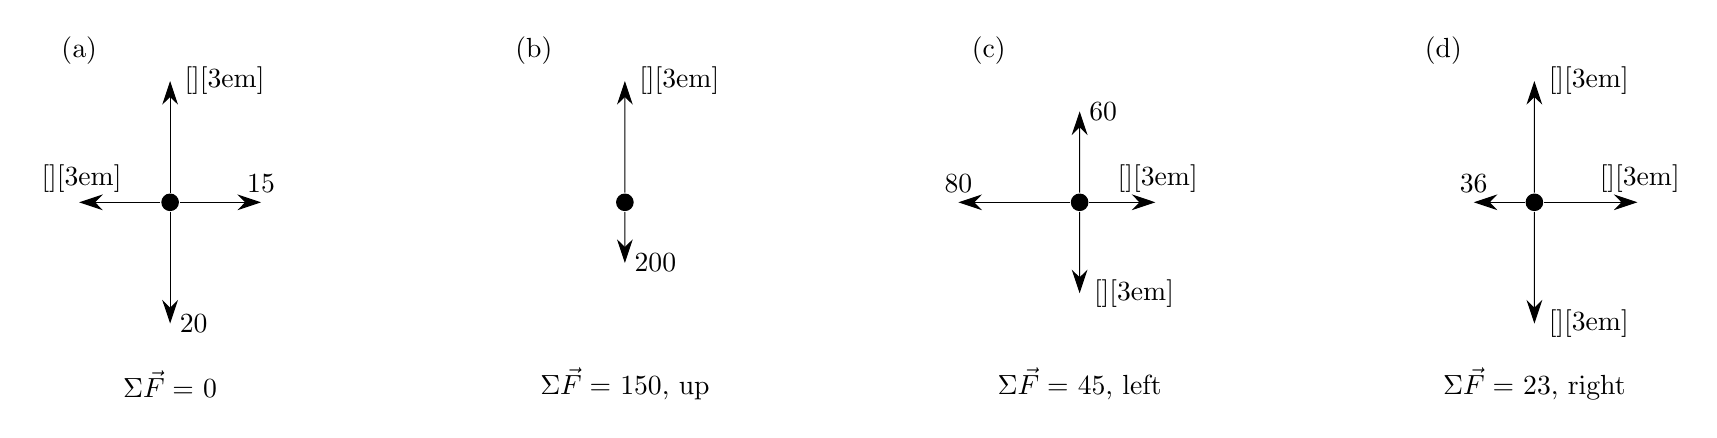
\begin{tikzpicture}[scale=0.77]
      \def\sep{7.5}

      \newcommand{\createFBD}[2]
        {
          \filldraw (a) circle [radius=0.136];
          \path (a) node {} 
            + (0,-3) node {
              $\Sigma\vec{F}=$ #2
            }
            + (-1.5,2.5) node {#1} ;
        }
      \newcommand{\forceblank}
        {\,\fillin[][3em]\SI{}{\newton}}


      \begin{scope}
        \node (a) at (0,0) {};
        \createFBD{(a)}{\SI{0}{\newton}}
        \vforce{  2 }{\forceblank}
        \vforce{ -2 }{\SI{20}{\newton}}
        \hforce{ 1.5}{\SI{15}{\newton}}
        \hforce{-1.5}{\forceblank}
      \end{scope}

      \begin{scope}
        \node (a) at (\sep,0) {};
        \vforce{  2 }{\forceblank}
        \vforce{ -1 }{\SI{200}{\newton}}
        \createFBD{(b)}{\SI{150}{\newton}, up}
      \end{scope}

      \begin{scope}
        \node (a) at (2*\sep,0) {};
        \createFBD{(c)}{\SI{45}{\newton}, left}
        \vforce{  1.5 }{\SI{60}{\newton}}
        \vforce{ -1.5 }{\forceblank}
        \hforce{1.25}{\forceblank}
        \hforce{ -2 }{\SI{80}{\newton}}
      \end{scope}

      \begin{scope}
        \node (a) at (3*\sep,0) {};
        \createFBD{(d)}{\SI{23}{\newton}, right}
        \vforce{  2 }{\forceblank}
        \vforce{ -2 }{\forceblank}
        \hforce{ 1.7}{\forceblank}
        \hforce{ -1 }{\SI{36}{\newton}}
      \end{scope}

    \end{tikzpicture}
  \end{EnvUplevel}

\pagebreak

\question
  Fill in the blanks in each of the situations depicted 
  below.  Draw the net force.

  \begin{center}  
    \begin{tikzpicture}[scale=0.7]
      \newcommand{\createFBD}[4]
        {
          \filldraw (a) circle [radius=0.15];
          \path (a) node {} 
            + (-5,2.5) node {#1}
            ++ (-1,-3.5) node[anchor=east] {$m=$}
            ++ (0,  0) node[anchor=west] {#2}
            ++ (0,-.8) node[anchor=east] {$a=$}
            ++ (0,  0) node[anchor=west] {#3}
            ++ (0,-.8) node[anchor=east] {$\Sigma\vec{F}=$ }
            ++ (0,-.2) node[anchor=west] {#4}
            ;
        }
      \newcommand{\makeblank}{\fillin[][3em]{} }

      \newcommand{\forceblank}
        {\,\makeblank N}

      \draw[dashed] (0,7) -- (0,-10);
      \draw[dashed] (14,-1.5) -- (-16,-1.5);


      \begin{scope}
        \node (a) at (-9,5) {};
        \createFBD
          {(a)}{3 kg}{\makeblank m/s$^2$, \makeblank}{23 N, right}
        \vforce{  2 }{\forceblank}
        \vforce{ -2 }{29.4 N}
        \hforce{ 3.5}{\forceblank}
        \hforce{ -1}{5 N}

      \end{scope}

      \begin{scope}
        \node (a) at (6,5) {};
        \createFBD
          {(b)}{2 kg}{8 m/s$^2$, left}{\makeblank N, \makeblank}
        \vforce{  2 }{19.6 N}
        \vforce{ -2 }{\forceblank}
        \hforce{-1.8}{\forceblank}
      \end{scope}

      \begin{scope}
        \node (a) at (-9,-5) {};
        \createFBD
          {(c)}{5 kg}{12 m/s$^2$, left}{\makeblank N, \makeblank}
        \vforce{  2 }{49 N}
        \vforce{ -2 }{\forceblank}
        \hforce{  3   }{7 N}
        \hforce{ -5   }{\forceblank}
      \end{scope}

      \begin{scope}
        \node (a) at (6,-5) {};
        \createFBD
          {(d)}{3 kg}{18 m/s$^2$, right}{\makeblank N, \makeblank}
        \vforce{  2.5 }{\forceblank}
        \vforce{ -2.5 }{\forceblank}
        \hforce{  4   }{\forceblank}
        \hforce{  -2   }{17 N}
      \end{scope}
    \end{tikzpicture}
  \end{center}


\question A 900-kg car accelerates from rest to 45~m/s in 6.8~seconds.  Fill in the free-body diagram below, assuming that the average force against the motion of the car due to air drag and friction is \SI{4900}{N}.

\begin{center}
  \begin{tikzpicture}
    \newcommand{\forceblank}
        {\,\fillin[][3em]\SI{}{\newton}}
    \filldraw (0,0) node (a) {}
      circle [radius=0.15];
    \vforce{  1.5 }{\forceblank}
    \vforce{ -1.5 }{\forceblank}
    \hforce{  4 }{\forceblank}
    \hforce{ -3 }{4900 N}
  \end{tikzpicture}
\end{center}

\vs \hrule \vs 

\question Consider 15,000-kg rocket that is accelerating upward at \SI{18.2}{m/s^2}.  Fill in the forces on the free-body diagram below.

\begin{center}
  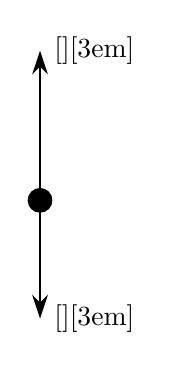
\begin{tikzpicture}
    \newcommand{\forceblank}
        {\,\fillin[][3em]\SI{}{\newton}}
    \filldraw (0,0) node (a) {}
      circle [radius=0.15];
    \vforce{  1.9 }{\forceblank}
    \vforce{ -1.5 }{\forceblank}
  \end{tikzpicture}
\end{center}

\end{questions}
\end{document}